\documentclass[uplatex, a4paper, 12pt, openany, oneside]{jsbook}

\usepackage[dvipdfmx]{graphicx}
\usepackage[dvipdfmx]{color}
\usepackage[dvipdfmx, bookmarks=true, setpagesize=false, hidelinks]{hyperref}
\usepackage{pxjahyper}

\usepackage{amsmath} % 数式パッケージを追加
\usepackage{amssymb} % 数学記号パッケージを追加

\usepackage{thesis}
\usepackage{here}
\usepackage{url}


\thesis{卒 業 論 文}
\title{
  \centering
  \scalebox{1.0}{自律移動ロボット用の雨天シミュレータの開発}
  \vspace{-0.3zh}
  \scalebox{1.0}{(検出された雨粒の時間間隔のモデル化)}
  %\vspace{-0.6zh} 
  \scalebox{0.6}{Development of a Rainy Weather Simulator for Autonomous Mobile Robots}\\
  %\vspace{-0.2zh}
  \scalebox{0.6}{(Modeling the Temporal Intervals of Detected Raindrops)}\\
  \vspace{-6zh}
}

\setlength{\textwidth}{\fullwidth}
\setlength{\evensidemargin}{\oddsidemargin}

\date{\today}
\vspace{-15.0zh}
\teacher{林原 靖男 教授}
\vspace{-15.0zh}
\organization{千葉工業大学 先進工学部 未来ロボティクス学科}
\author{21C1131 柳大地}
\vspace{-15zh}

\renewcommand{\baselinestretch}{1.2}
\begin{document}

%% Front Matter
\frontmatter{}
%
\maketitle
%
%!TEX root = ../thesis.tex
\chapter*{概要}
\thispagestyle{empty}
%
\begin{center}
  \scalebox{1.5}{自律移動ロボット用の雨天シミュレータの開発}\\
  \scalebox{1.5}{(検出された雨粒の時間間隔のモデル化)}
  \vspace{1.0zh}
\end{center}
\vspace{1.0zh}
%

%
近年,自律移動ロボットは幅広い産業分野で需要が高まっており屋外で雨天においても自律移動できることが望まれている.
本研究室では,2D LiDARを搭載した屋外自律移動ロボットを研究・開発している.
しかし,雨天環境での自律移動はLiDARが雨粒を検出し停止,回避動作を行うことにより困難である.
先行研究\cite{mura}では雨天のLiDARデータを取得し,取得したデータを解析,モデル化した.
しかし,取得したデータが少ないことや雨粒の時間間隔のモデル化ができていない.
本論文では,先行研究で不足する雨天時のLiDARデータの追加取得,雨粒の時間間隔のモデル化を行い,自律移動ロボット用の雨天シミュレータの開発を行った.
シミュレータでは雨粒の距離のモデル化に基づいた雨を再現することができた.
%
%
%
%
%
%
%
%
%
%
%
%
%

\vspace{2.0zh}
キーワード: 2DLiDAR,雨天,シミュレータ
%

\newpage
%%
\chapter*{abstract}
\thispagestyle{empty}
%
\begin{center}
  \scalebox{1.3}{Development of a Rainy Weather Simulator for Autonomous Mobile Robots}
  \scalebox{1.3}{(Modeling the Temporal Intervals of Detected Raindrops)}
\end{center}
\vspace{1.0zh}
%
In recent years, the demand for autonomous mobile robots has been increasing across various industrial sectors, with the capability to operate autonomously outdoors even in rainy weather being highly desirable.  
In our laboratory, we are engaged in the research and development of outdoor autonomous mobile robots equipped with 2D LiDAR.
However, achieving autonomous navigation in rainy conditions is challenging due to LiDAR detecting raindrops, leading to unintended stops or avoidance maneuvers.  
In prior research by Murabayashi [1], LiDAR data in rainy conditions was collected, analyzed, and modeled. 
However, the amount of collected data was insufficient, and the temporal modeling of raindrops was not addressed.  
This paper focuses on supplementing the insufficient rainy weather LiDAR data from previous studies and modeling the temporal intervals of raindrops.
Based on these efforts, a rainy weather simulator for autonomous mobile robots was developed.
The simulator successfully reproduces rainfall based on the modeled distance of raindrops.
%
\vspace{2.0zh}

keywords: 2D LiDAR, rainyweather, simulator
%
\tableofcontents
%
\listoffigures
%
\listoftables
%

%
%% Main Matter
\mainmatter{}
%
\chapter{序論}
\label{chap:introduction}
%
%\input{introduction/preface}
%
%!TEX root = ../thesis.tex

\section{背景}
近年,自律移動ロボットは幅広い産業分野で需要が高まっており屋外で雨天においても自律移動できることが望まれている.
しかし,雨天環境での自律移動はLiDARが雨粒を検出し停止,回避動作を行うことにより困難である.
本研究室では,2D LiDARを搭載した屋外自律移動ロボットを研究・開発している.
雨天時の自律移動に関連する研究では雨粒を模擬または,実環境で行っている.
先行研究\cite{mura}では噴霧器で雨天を模擬した環境と雨天環境の比較を行ったが実際の雨天を十分に再現することはできなかった.
そのため,様々な雨量の環境をシミュレートできるシステムが望まれていると考え,雨天時の2DLiDARデータのモデル化を行った.

\section{目的}
本研究は先行研究\cite{mura}を発展させ,新たに解析及びモデル化を行い,2DLiDARが検出する雨をシミュレータ上で再現することを目的とする.

\section{先行研究}
村林\cite{mura}は,2D LiDARが検出する雨をシミュレータ上で再現し,ロボットの自律移動を検証できるシステムを構築するため,雨天時の2D LiDARデータの取得,解析,モデル化を行った.
コンピュータ内で雨天シミュレータを構築するためには,解析内容として「検出された雨粒の距離の分布」「検出された雨粒の時間間隔の分布」「隣り合うレーザで検出された雨粒の距離の分布」のモデル化が必要であると述べている.
これにより,22件の雨天時の2D LiDARデータの取得,「検出された雨粒の距離の分布」「隣り合うレーザで検出された雨粒の距離の分布」を正規近似し,求められた平均距離と標準偏差を一次近似によりモデル化した.

\begin{figure}[h]
  \centering
  \includegraphics[keepaspectratio, scale=0.08]{images/png/rain_robot_wall2.png}
  \caption{2D LiDAR data acquisition experiment in rainy weather (sourse:\cite{mura})}
  \label{Fig:1.1}
\end{figure}

\begin{figure}[h]
  \centering
  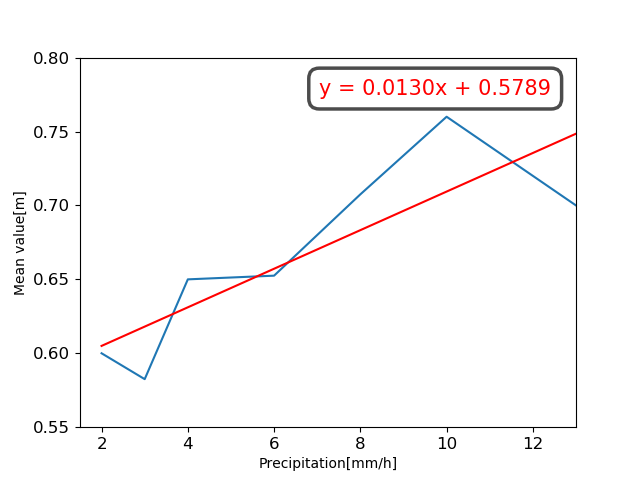
\includegraphics[keepaspectratio, scale=0.38]{images/png/4_3mean_kinji.png}
  \caption{Relationship between the amount of precipitation and the average distance over which the same raindrop was detected (sourse:\cite{mura})}
  \label{Fig:1.2}
\end{figure}

\begin{figure}[h]
  \centering
  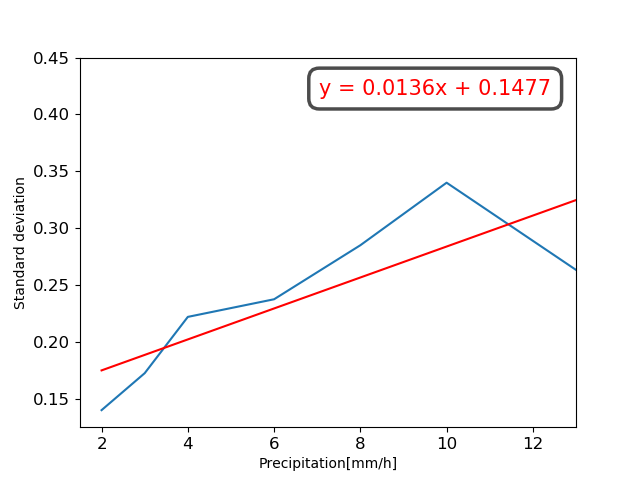
\includegraphics[keepaspectratio, scale=0.38]{images/png/4_3std_kinji.png}
  \caption{Relationship between the amount of precipitation and the standard deviation of the distance over which the same raindrops are detected (sourse:\cite{mura})}
  \label{Fig:1.3}
\end{figure}


\newpage
\section{論文の構成}
本論文は以下のように構築される.第1章では,本研究の背景,目的,先行研究を述べる.
第2章では,本研究に関連する要素技術を述べる.
第3章では,雨天時の2DLiDARデータの追加取得実験について目的,実験装置,方法,結果について述べる.
第4章では,検出された雨粒の時間間隔のモデル化について近似手法,結果,考察を述べる.
第5章では,解析,モデル化したデータを基に開発した雨天シミュレータについて結果と考察を述べる.
第6章では,本論文の結論と今後の展望を述べる.


%


%ここにディレクトリのパスを追加していく
\chapter{要素技術}
\label{chap:technology}

\section{2D LiDAR}

2D LiDAR(Light Detection and Ranging)は,レーザ光を照射することで周囲の物体までの距離を計測し主に自動運転やロボティクスなどで活躍している.
レーザ光を特定の平面内で回転させることで一定の角度ごとに照射し,物体からの反射光を受信し距離を算出する.

本研究で使用する2D LiDARをfigに示す.
このLiDARにはurg-nodeパッケージが提供されており2D LiDARが取得する角度を変更することが可能である.

\section{Rviz}

Rvizはロボットが収集したセンサデータを視覚的に表示するアプリケーションである.

本研究では取得した雨天の2D LiDARデータとシミュレータに追加したノイズの可視化をした.
\chapter{雨天時の2D LiDARデータの追加取得}

\label{chap:experiments}

\section{実験目的}

先行研究\cite{mura}と同様の実験を行い様々な雨量の雨天環境の2D LiDARデータを取得することを目的とする.

\section{実験装置}

実験装置は先行研究\cite{mura}と同様である.
実験装置として本研究室で開発しているロボットORNE-box2\cite{orne}を使用する.
ロボットの外観と仕様を\figref{Fig:4.1}と\tabref{table:ORNE-box2}に示す.
また,使用した2D LiDAR(UTM-30LX-EW)の外観と仕様を\figref{Fig:4.2}と\tabref{table:angular}に示す.

\begin{figure}[H]
  \centering
  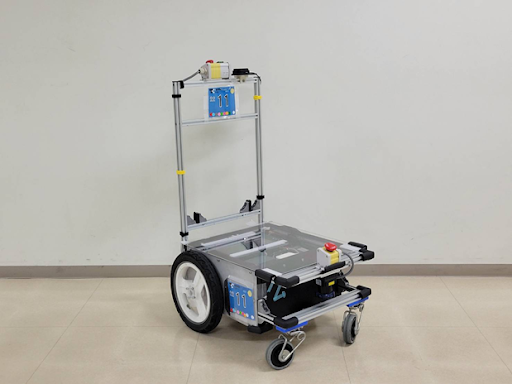
\includegraphics[keepaspectratio, scale=0.4]{images/png/orne-box2.png}
  \caption{ORNE-box2(source:\cite{mura})}
  \label{Fig:4.1}
\end{figure}

\newpage
\vspace{10zh}

\begin{table}[H]
  \centering
  \caption[Specifications of ORNE-box2]{Specifications of ORNE-box2(source:\cite{mura}\cite{orne})}
  \begin{tabular}{|l|l|}
  \hline
  Depth {[}mm{]}          & 600 \\ \hline
  Width {[}mm{]}          & 507 \\ \hline
  Height {[}mm{]}         & 957 \\ \hline
  Wheel diameter {[}mm{]} & 304 \\ \hline
  Weight {[}kg{]}         & 30  \\ \hline
  \end{tabular}
  \label{table:ORNE-box2}
  \end{table}

\vspace{10zh}
\begin{figure}[H]
  \centering
  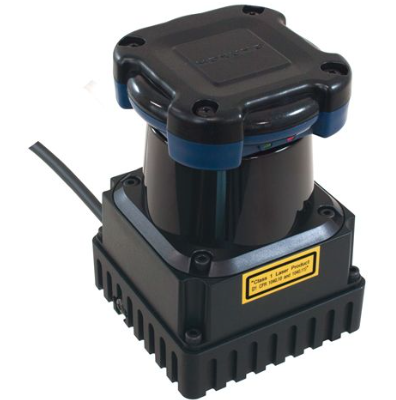
\includegraphics[keepaspectratio, scale=0.6]{images/png/LiDAR.png}
  \caption{2D LiDAR(UTM-30LX-EW)(source:\cite{lidar})}
  \label{Fig:4.2}
\end{figure}


  \begin{table}[H]
    \small
    \centering
    \caption[Specifications of Hokuyo UTM-30LX-EW]{Specifications of Hokuyo UTM-30LX-EW\cite{lidar}(source:\cite{mura}\cite{lidar})}
    \label{table:angular}
    \begin{tabular}{|l|l|}
    \hline
    Light Source        & \begin{tabular}[c]{@{}l@{}}Semiconductor Laser(λ = 905nm)\\Laser class 1 (FDA)\end{tabular} \\ \hline
    Supply Voltage      & DC12V ± 10\%   \\ \hline
    Supply Current      & 700mA or less (1A during startup)  \\ \hline
    Detection Range and Object & \begin{tabular}[c]{@{}l@{}}Guaranteed Range:0.1〜30m (White Kent Sheet)\\ Maximum Range:60m (Measurement limit)\\ Minimum detection width:130mm at 10m(Varies with distance)\end{tabular} \\ \hline
    Measurement Accuracy      & \begin{tabular}[c]{@{}l@{}}0.1m〜10m:± 30mm,10m〜30m:± 50mm(White Kent Sheet)\\ Ambient light below 3000lx:0.1〜10m:± 30mm(White Kent Sheet)\\ Ambient light below 10000lx:0.1〜10m:± 50mm(White Kent Sheet)\end{tabular} \\ \hline
    Scan Angle      & 270°  \\ \hline
    Angular Resolution     & Approx. 0.25° (360°/1440 divisions) \\ \hline
    Scan rate     & 25ms/scan  \\ \hline
    Interface  & Ethernet 100BASE-TX (Auto-negotiation) \\ \hline
    Protective Structure      & IP67 (IEC Standard) \\ \hline
    \end{tabular}
    \end{table}
  \clearpage

\section{実験方法}
実験方法は概ね先行研究\cite{mura}と同様である.
先行研究\cite{mura}にてロボットと壁の距離の関係性は確認されなかったため,5mに固定し実験を行った.
実験場所を\figref{Fig:4.3}に示す.6号館と2号館通路突き当りの赤の矢印の場所で行った.
実験の様子を\figref{Fig:4.4}に示す.
壁よりも近い距離で物体が検出された場合,雨粒であると考えられる.

実験方法を以下に示す.
\begin{enumerate}
    \item ロボットを壁から5m離して配置する.
    \item 実験場所は千葉工業大学津田沼キャンパス.(\figref{Fig:4.3})
    \item \texttt{rosbag}を使用し,約2分間データを取得.
\end{enumerate}

\begin{figure}[H]
  \centering
  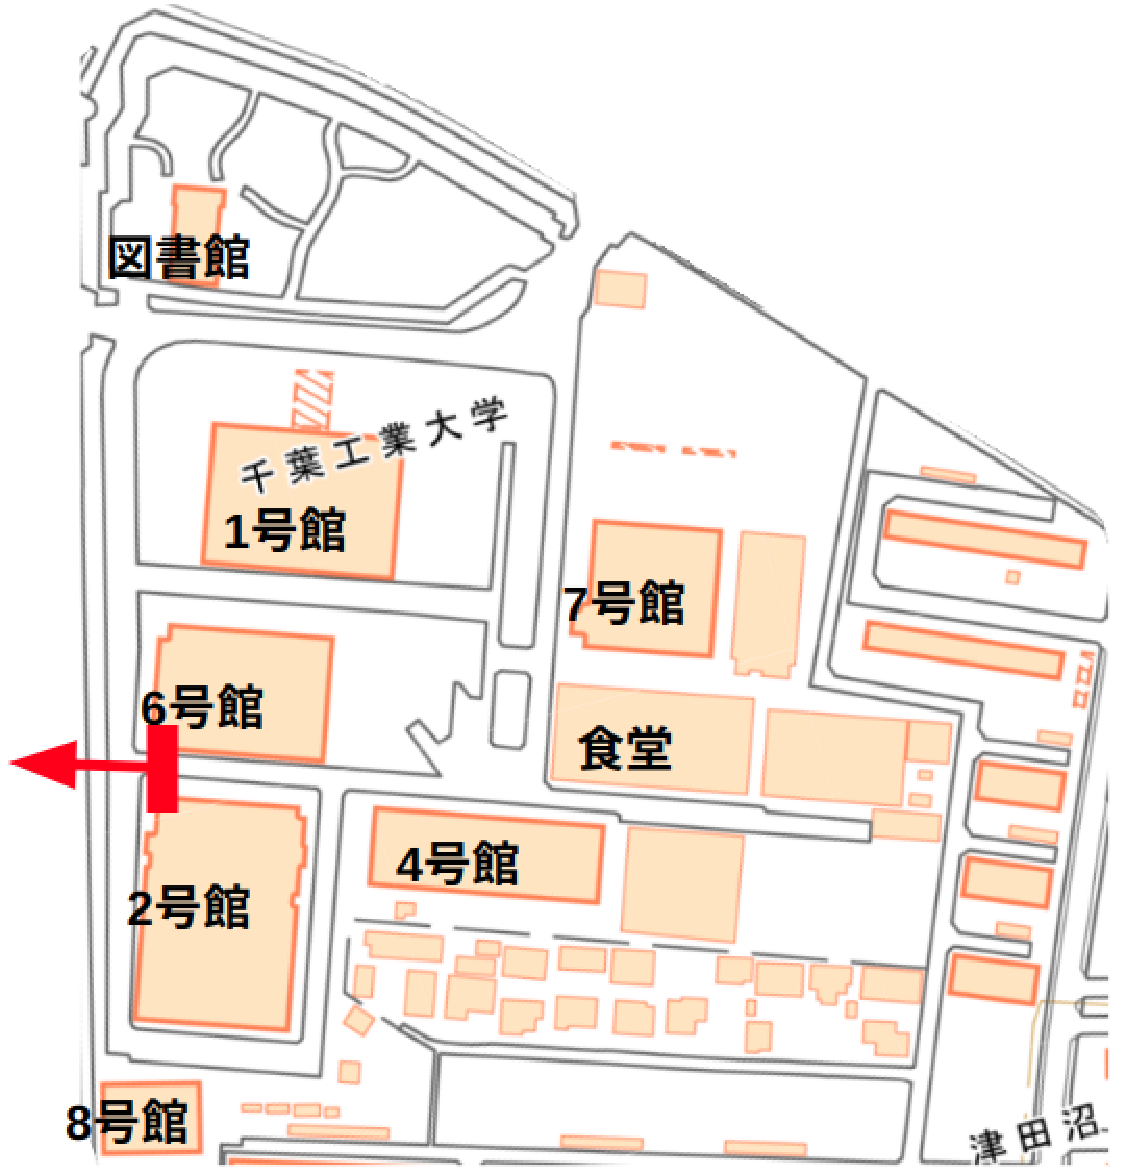
\includegraphics[keepaspectratio, scale=0.5]{images/png/ex_map3.pdf}
  \caption{Experiment location(source:\cite{mura})}
  \label{Fig:4.3}
\end{figure}

\begin{figure}[H]
  \centering
  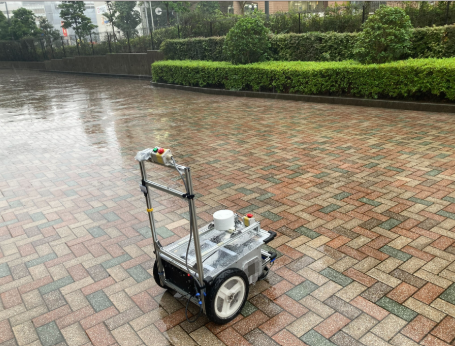
\includegraphics[keepaspectratio, scale=0.7]{images/png/ex.png}
  \caption{Experimental Setup}
  \label{Fig:4.4}
\end{figure}

\section{実験結果}
追加取得したデータ数を\tabref{table:Additional_number_of_data_acquired}に示す.
先行研究\cite{mura}と合わせたデータ数を\tabref{table:Total_number_of_data_acquired}に示す.
先行研究\cite{mura}同様に雨量が多いほど雨粒が頻繁に検出された.

\begin{table}[htbp]
  \centering
  \footnotesize
  \caption{The number of additional data points acquired under rainy weather conditions}
  \label{table:Additional_number_of_data_acquired}
  \begin{tabular}{|l|l|r|}
  \hline
  Rainfall & \multicolumn{1}{l|}{Number of data} \\
  \hline
  Range: 2.0 to 13 mm/h & 8 \\
  \hline
  \end{tabular}
\end{table}

\begin{table}[htbp]
  \centering
  \footnotesize
  \caption{The total number of data points acquired under rainy weather conditions.}
  \label{table:Total_number_of_data_acquired}
  \begin{tabular}{|l|l|r|}
  \hline
  Rainfall & \multicolumn{1}{l|}{Number of data} \\
  \hline
  Range: 2.0 to 13 mm/h & 30 \\
  \hline
  \end{tabular}
\end{table}
\chapter{検出された雨粒の時間間隔のモデル化}

\label{chap:raincycle}

先行研究\cite{mura}では雨粒の時間間隔の分布をヒストグラムで表したが近似式を求められていない.
したがって,先行研究\cite{mura}のヒストグラムをガンマ分布を用い近似を行った.

\section{ガンマ分布}
ガンマ分布の定義と性質を以下に示す.chatgpt\cite{gpt}で作成した文書を基に作成している.
ガンマ分布は連続確率分布の一種であり,形状パラメータ \( k > 0 \) と尺度パラメータ \( \theta > 0 \) によって定義される.確率密度関数 (PDF) は以下の式で表せる:

\begin{equation}
f(x; k, \theta) = \frac{x^{k-1} e^{-x/\theta}}{\Gamma(k) \theta^k}, \quad x > 0,
\end{equation}

ここで,\(\Gamma(k)\) はガンマ関数と呼ばれ,次式で定義される:

\begin{equation}
\Gamma(k) = \int_{0}^{\infty} t^{k-1} e^{-t} \, dt.
\end{equation}

ガンマ分布は形状パラメータ \( k \) によって分布の形状が変わり,尺度パラメータ \(\theta\) によってスケールが調整される.

\subsection{基本的性質}
ガンマ分布の平均と分散は以下のように表せる:
\vspace{3zh}
\begin{itemize}
    \item 平均:\(\mathbb{E}[X] = k \theta\)
    \item 分散:\(\mathrm{Var}(X) = k \theta^2\)
\end{itemize}

\vspace{10zh}
\section{検出された雨粒の時間間隔の分布}
取得した降水量2〜13mm/hの取得データをガンマ分布で近似した例を\figref{Fig:5.1}〜\figref{Fig:5.6}に示す.
下記の図はx軸が降水量,y軸が対応する確率密度を表している.
先行研究同様,降水量が少ないほどデータ数が減少していく傾向であった.
形状パラメータは降水量による関連性は見られなかった.このことから,降水量によって分布の形状は変化しない可能性があると考えられる.
一方,尺度パラメータは降水量が増えるほど減少していく傾向が見られた.このことから,降水量が増えるほどデータのばらつきが小さくなる傾向があると考えられる.
\vspace{7.0zh}

\begin{figure}[H]
    \centering
    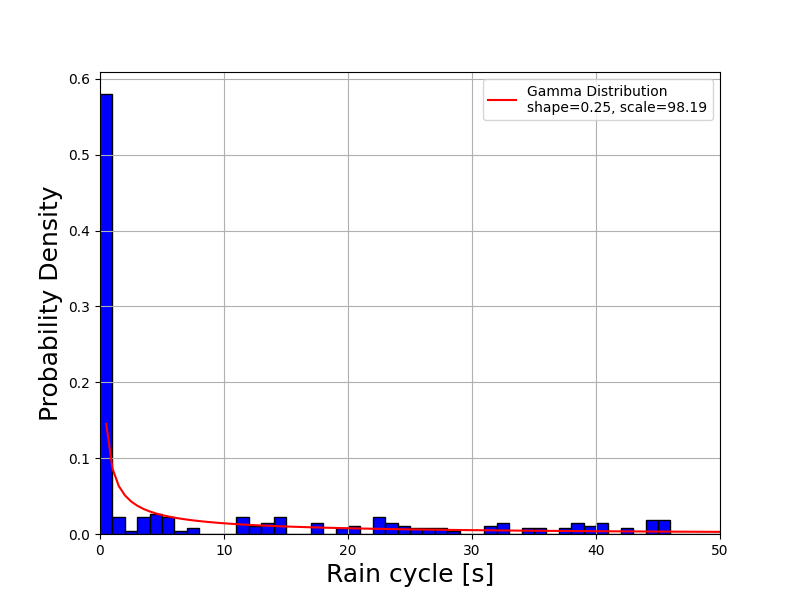
\includegraphics[keepaspectratio, scale=0.5]{images/png/3mm.png}
    \caption{Time interval distribution of detected raindrops (2mm/h)}
    \label{Fig:5.1}
\end{figure}

\begin{figure}[H]
    \centering
    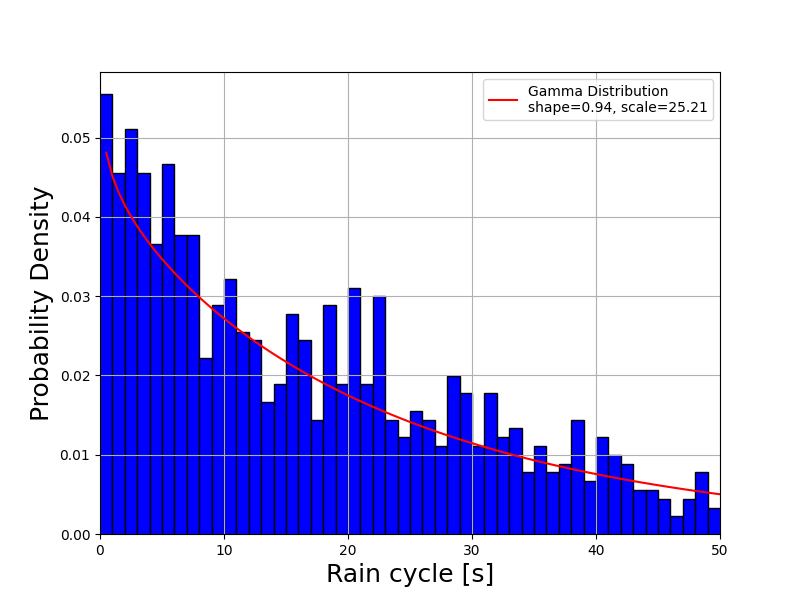
\includegraphics[keepaspectratio, scale=0.5]{images/png/4mm.png}
    \caption{Time interval distribution of detected raindrops (4mm/h)}
    \label{Fig:5.2}
\end{figure}

\begin{figure}[H]
    \centering
    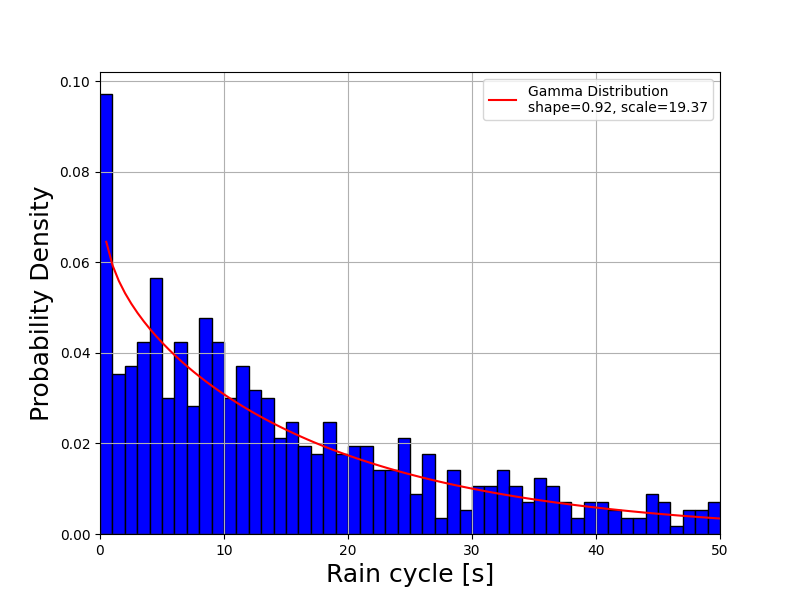
\includegraphics[keepaspectratio, scale=0.5]{images/png/6mm.png}
    \caption{Time interval distribution of detected raindrops (6mm/h)}
    \label{Fig:5.3}
\end{figure}

\begin{figure}[H]
    \centering
    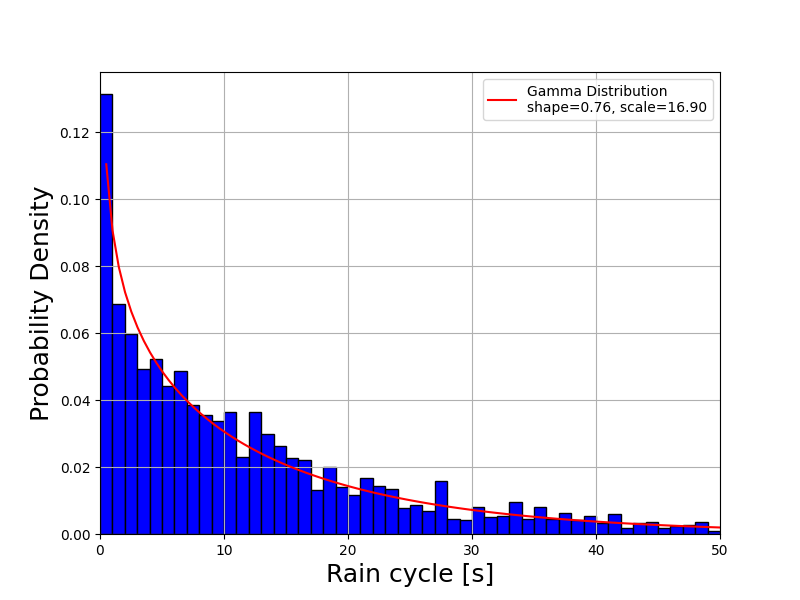
\includegraphics[keepaspectratio, scale=0.5]{images/png/8mm.png}
    \caption{Time interval distribution of detected raindrops (8mm/h)}
    \label{Fig:5.4}
\end{figure}

\begin{figure}[H]
    \centering
    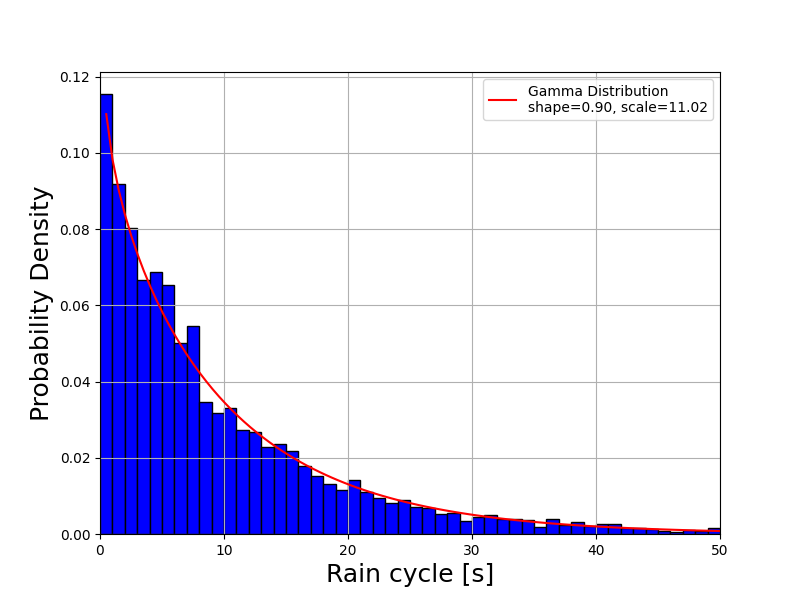
\includegraphics[keepaspectratio, scale=0.5]{images/png/10mm.png}
    \caption{Time interval distribution of detected raindrops (10mm/h)}
    \label{Fig:5.5}
\end{figure}

\begin{figure}[H]
    \centering
    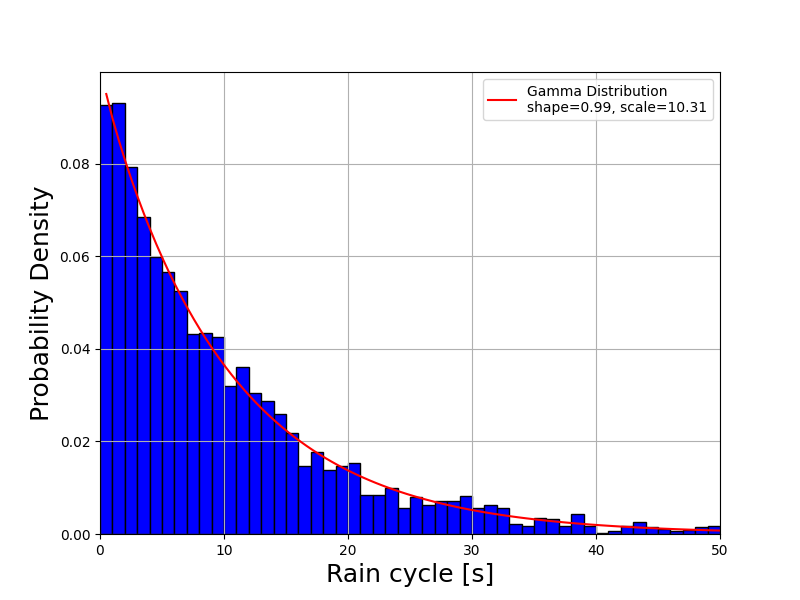
\includegraphics[keepaspectratio, scale=0.5]{images/png/13mm.png}
    \caption{Time interval distribution of detected raindrops (13mm/h)}
    \label{Fig:5.6}
\end{figure}

\section{モデル化}
前節で得た様々な降水量のガンマ分布の近似を基にモデル化を行った.
平均値と降水量の関係を\figref{Fig:5.7}に示す.
また,標準偏差と降水量の関係を\figref{Fig:5.8}に示す.
降水量が増えるほど平均値,標準偏差共に減少していく傾向があることが分かった.
このことから,降水量が増えるほど雨粒の時間間隔が短くなり,ばらつきが小さくなると考えられる.


\begin{figure}[H]
    \centering
    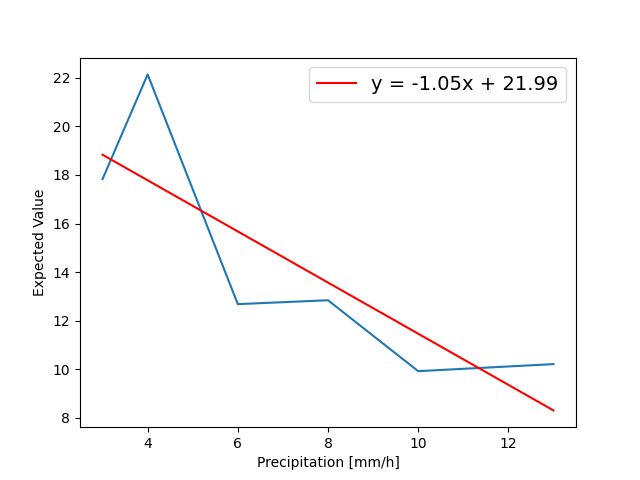
\includegraphics[keepaspectratio, scale=0.5]{images/png/kitaiti.png}
    \caption{Average value of the time interval distribution of detected raindrops}
    \label{Fig:5.7}
\end{figure}

\begin{figure}[H]
    \centering
    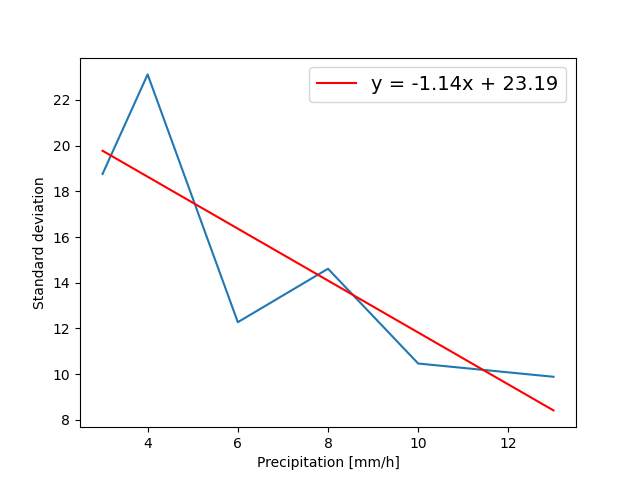
\includegraphics[keepaspectratio, scale=0.5]{images/png/hyouzunhensa.png}
    \caption{Standard deviation of the time interval distribution of detected raindrops}
    \label{Fig:5.8}
\end{figure}
\chapter{雨天シミュレータの開発}

\label{chap:simulator}

先行研究\cite{mura}及び前章で得られた解析結果とモデル化を活用することで,雨天環境をシミュレータ上で再現可能であると考えられる.
本論文では,「検出された雨粒の距離の分布」に基づいて雨を再現した.
しかし,「検出された雨粒の時間間隔の分布」や「隣接するレーザーで検出された雨粒の距離の分布」については未だ組み込まれていない.
これらを追加することで,実環境により近い,様々な雨量の雨粒を再現できると期待される.

\section{シミュレータ環境}
シミュレータ環境はGazebo\cite{gaze}である.
本研究室で開発されたornebox simulator\cite{simu}をベースに開発を行った.
シミュレータ内のLiDARが検出する距離に雨を模したノイズを追加することで,雨天環境を再現した.

\section{シミュレーション結果}
「検出された雨粒の距離の分布」で得た平均値と標準偏差を基に雨を模したノイズを追加し雨天環境の再現を行った.
検出された雨粒の距離の分布を示す.
\chapter{結論}

\label{chap:conclusion}

\section{まとめ}
本研究では,先行研究\cite{mura}を発展させ,雨天時の2DLiDARデータの追加取得,モデル化,シミュレータ開発を行った.
モデル化では,「検出された雨粒の時間間隔の分布」をガンマ分布を用い近似し,モデル化した.
シミュレータ開発では,「検出された雨粒の距離の分布」の平均値と標準偏差を用いることで雨粒を模したノイズを追加し,雨天環境を再現した.

\section{今後}
今後は「検出された時間間隔の分布」と「隣り合うレーザで検出された雨粒の距離の分布」の解析及びモデル化で得た式をシミュレータに組み込むことでより実環境に近い雨を再現できると考える.

%
%% Back Matter
\backmatter{}
%
%!TEX root = ../thesis.tex
%\bibliographystyle{plain}
\bibliographystyle{junsrt}
%\bibliography{report}
\nocite{*}
\bibliography{main_bibliography}
%
%!TEX root = ../thesis.tex
\chapter*{付録}
\addcontentsline{toc}{chapter}{付録}

%
%!TEX root = ../thesis.tex
\chapter*{謝辞}
\addcontentsline{toc}{chapter}{謝辞}

本研究を進めるにあたり,1年に渡り, 熱心にご指導を頂いた林原靖男教授に深く感謝いたします.
%


%

\end{document}
